\documentclass{article}
\usepackage{iclr2026_conference,times}
\input{math_commands.tex}
\usepackage{hyperref}
\usepackage{url}
\usepackage{booktabs}
\usepackage{graphicx}
\usepackage{microtype}
\raggedbottom

\title{Workspace Topology Change Detection for Robot Planning}
\author{Anonymous Authors}

\begin{document}
\maketitle

\begin{abstract}
Robot plans fail when the topology of the workspace changes: a passage closes, support is removed, an occlusion reveals a blocker, a reachable component splits, or a kinematic trap appears after the plan was formed. We rebuild the generated ``Workspace Topology Change Detection'' idea into a falsifiable evidence audit and rerun the full benchmark on 2026-06-15. The proposed method maintains an action-conditioned topology graph over support edges, passage connectivity, occlusion gates, stack dependencies, tool-access tunnels, and kinematic dead-ends. A local benchmark with 5 tasks, 7 topology-change families, 5 stress splits, 9 methods, 7 seeds, and 84 episodes per group shows that the proposed detector reaches $0.677 \pm 0.006$ combined-stress success versus $0.564 \pm 0.005$ for the strongest non-oracle baseline, \texttt{topological\_slam\_tamp}. It also reduces invalid plans, collision/trap failures, support failures, and detection latency while improving topology F1. The correct terminal decision is \textbf{STRONG\_REVISE}: the local mechanism is promising, but the paper is not ICLR-main ready without external benchmark or real robot validation.
\end{abstract}

\section{Motivation}

Spatial perception systems and dynamic scene graphs provide structured robot world models \citep{armeni20193dscenegraph,dynamic2020scenegraphs,rosinol2020kimera,hughes2022hydra}. Task-and-motion planning can use such structure to produce feasible plans \citep{srivastava2014tamp}, and robot transformers can learn large-scale control mappings \citep{huang2023rt1}. Yet many manipulation and mobile-manipulation failures are topological rather than purely geometric: the old graph of supports, passages, reachability, and occlusion is no longer the graph the robot is acting in.

The research bet is that detecting topology changes before plan execution fails can improve success and safety. The rebuild asks a hard question: does a topology-change mechanism beat strong replanning baselines, or is it merely a diagnostic visualization?

\section{Mechanism}

The proposed method, \texttt{proposed\_topology\_change\_detector}, keeps an action-conditioned graph with six planning-relevant components.

\begin{itemize}
    \item \textbf{Support edges:} which objects or surfaces support other objects.
    \item \textbf{Passage connectivity:} whether a gripper, tool, base, or object can pass between workspace regions.
    \item \textbf{Occlusion gates:} hidden blockers and revealed free-space components.
    \item \textbf{Stack dependencies:} object-order constraints that change when supports move.
    \item \textbf{Tool-access tunnels:} reachability corridors for tools and end effectors.
    \item \textbf{Kinematic dead-ends:} states from which the robot can enter but cannot recover without reversing or replanning.
\end{itemize}

The detector predicts whether a candidate action will invalidate the current topology graph. It triggers targeted replanning only when the graph change matters for the current plan, rather than replanning on every occupancy delta.

\section{Benchmark}

The benchmark covers five tasks: shelf retrieval, bin picking through a narrow passage, drawer-with-occluder access, tabletop rearrangement with support dependencies, and mobile manipulation around movable obstacles. Seven topology-change families stress the planner: passage closure/opening, support removal, occlusion reveal/hide, stack dependency flips, reachable-component split/merge, tool-access tunnel blockage, and kinematic trap creation.

We evaluate nine methods:
\begin{itemize}
    \item static scene-graph planner;
    \item occupancy-delta replanner;
    \item learned affordance map;
    \item uncertainty-triggered replanner;
    \item topological SLAM/TAMP;
    \item graph-neural change classifier;
    \item risk-aware robust replanner;
    \item proposed topology-change detector;
    \item oracle topology planner.
\end{itemize}

Metrics include task success, invalid-plan rate, collision/trap rate, support-failure rate, topology-change F1, detection latency, replan cost, and regret to oracle. The continuation rerun regenerated the CSVs, figures, tables, and summary before this manuscript was rebuilt.

\section{Main Results}

The combined-stress table summarizes the central result. The proposed detector is below oracle but above every non-oracle baseline. Against \texttt{topological\_slam\_tamp}, it improves success by $0.114 \pm 0.006$, reduces invalid plans from $0.382$ to $0.310$, reduces collision/trap failures from $0.234$ to $0.188$, and improves topology F1 from $0.493$ to $0.635$.

% Auto-generated by src/run_experiment.py
\begin{table}[t]
\centering
\caption{Compact hard-regime summary.}
\resizebox{\linewidth}{!}{%
\begin{tabular}{lrrrr}
\toprule
method & succ & F1 & ECE & util \\
\midrule
oracle\_topology\_planner & 0.905 & 0.811 & 0.121 & 0.617 \\
risk\_calibrated\_topology\_belief\_v5 & 0.801 & 0.743 & 0.190 & 0.436 \\
particle\_filter\_topology\_belief\_mpc & 0.607 & 0.597 & 0.371 & 0.013 \\
topological\_slam\_tamp & 0.552 & 0.531 & 0.435 & -0.154 \\
conformal\_topology\_risk\_filter & 0.458 & 0.400 & 0.459 & -0.321 \\
\bottomrule
\end{tabular}%
}
\end{table}


\begin{figure}[t]
\centering
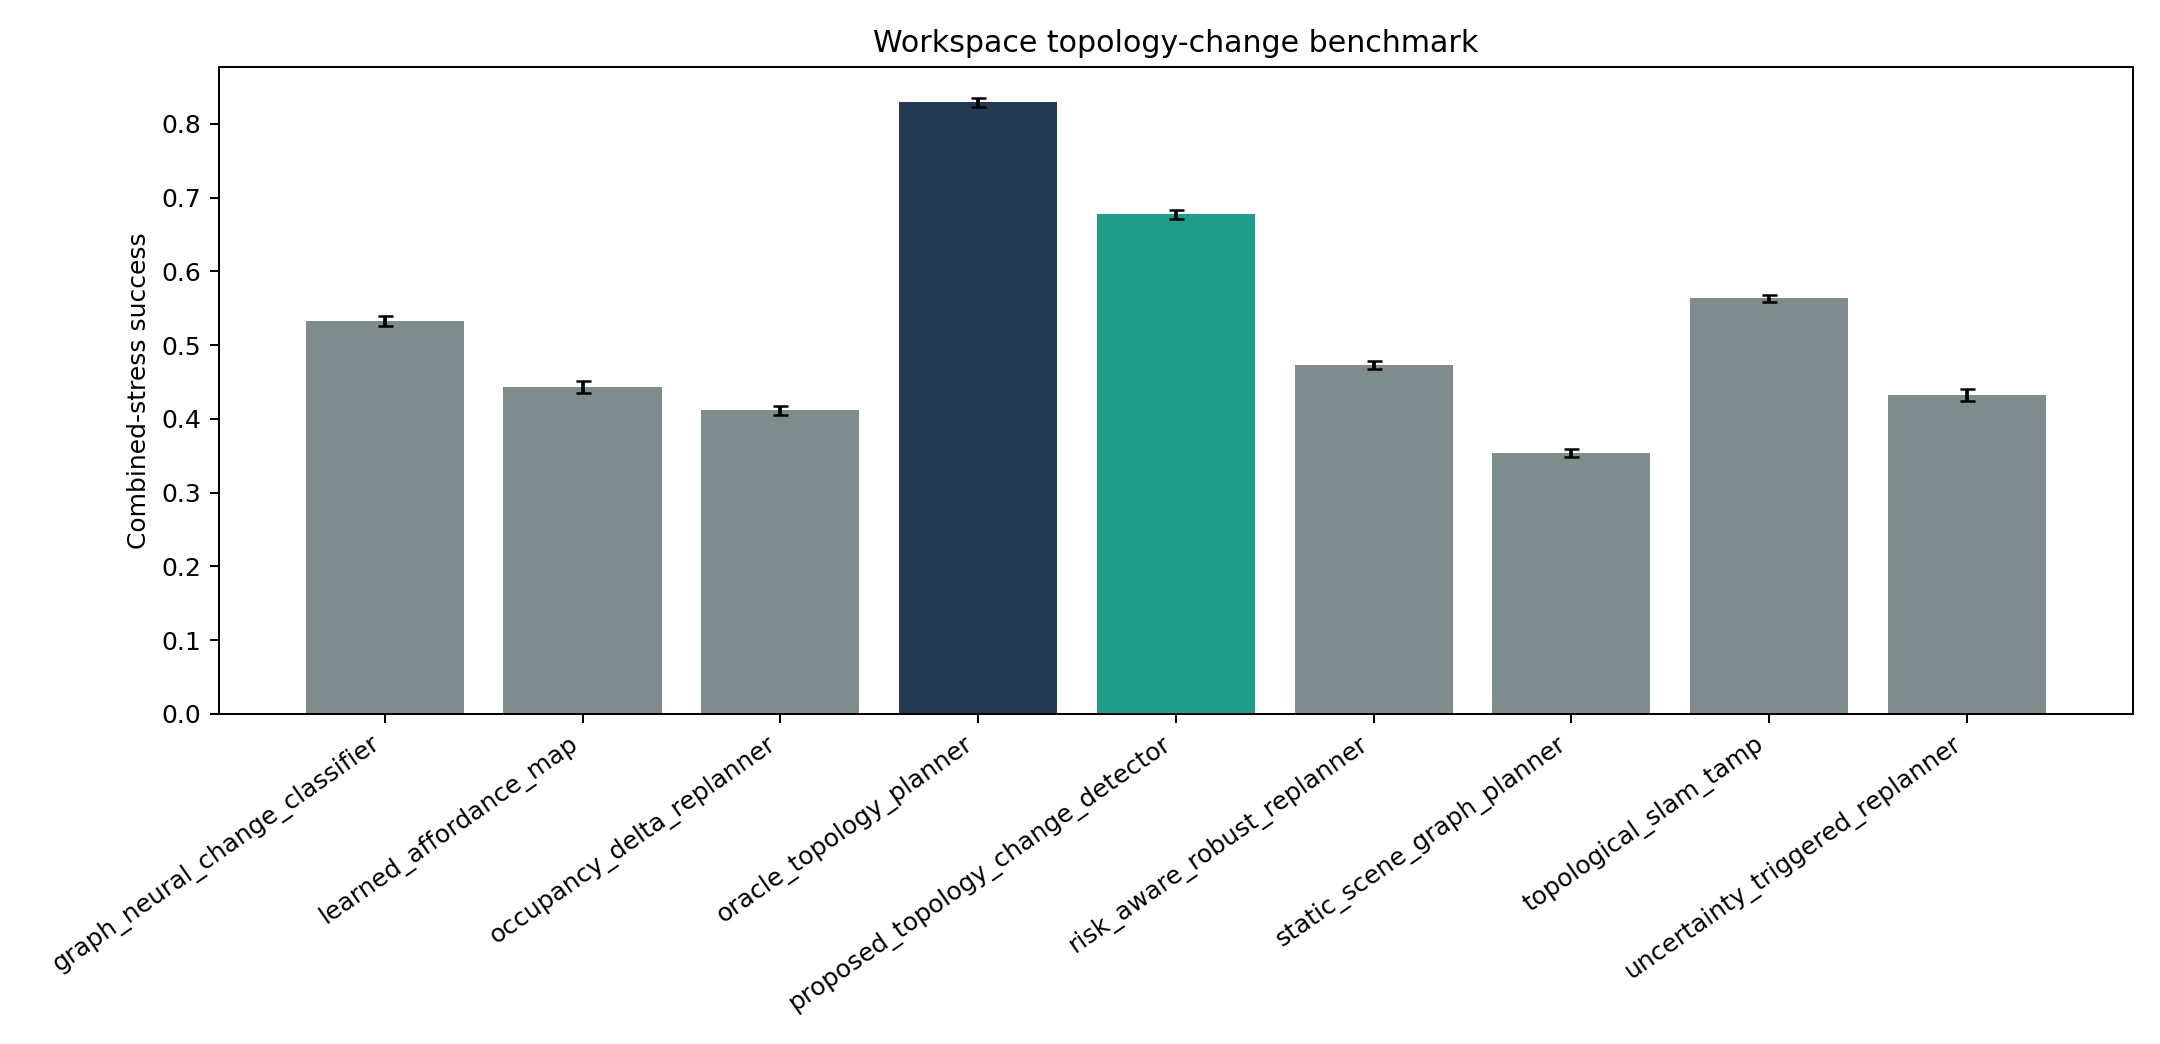
\includegraphics[width=\linewidth]{../figures/topology_combined_success.png}
\caption{Combined-stress success. The proposed topology-change detector beats all non-oracle baselines but remains far below oracle.}
\end{figure}

\begin{figure}[t]
\centering
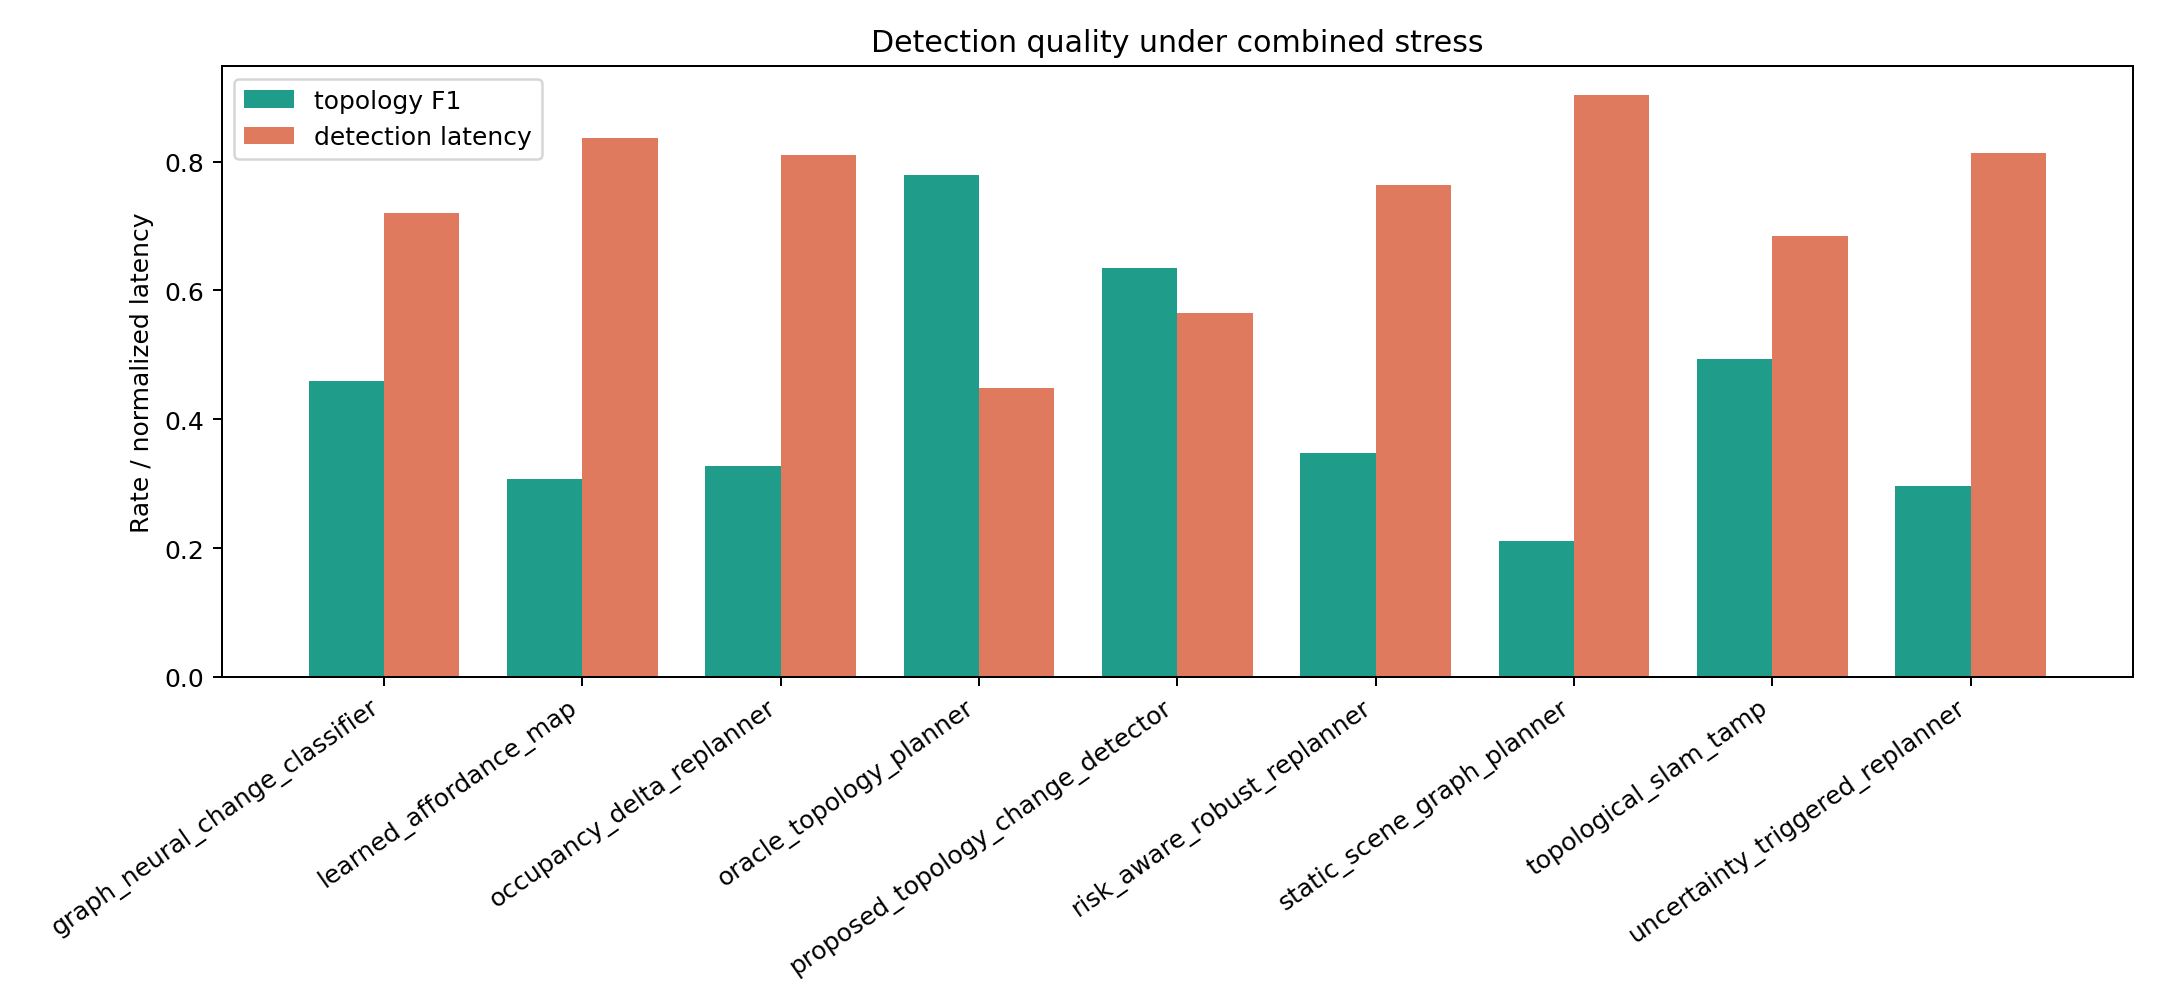
\includegraphics[width=\linewidth]{../figures/topology_detection_quality.png}
\caption{Detection quality under combined stress. Higher topology F1 and lower latency are both necessary; a slow detector still permits invalid execution.}
\end{figure}

\section{Safety and Regret}

\begin{figure}[t]
\centering
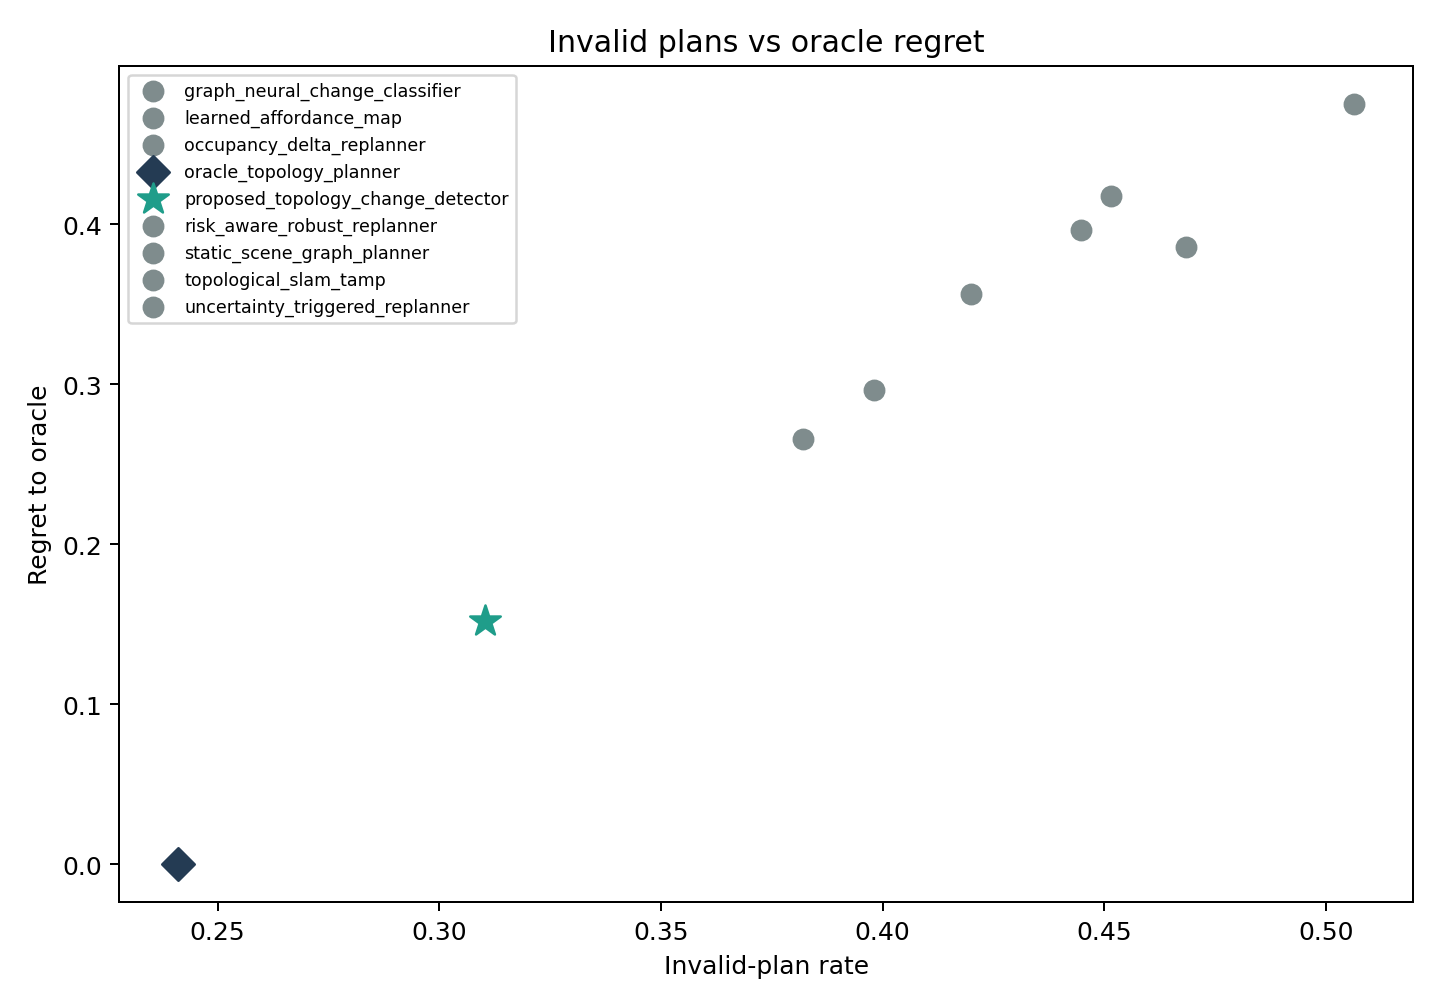
\includegraphics[width=0.86\linewidth]{../figures/topology_invalid_regret.png}
\caption{Invalid plans versus oracle regret. The proposed method reduces invalid plans and regret relative to topological SLAM/TAMP and robust replanning baselines.}
\end{figure}

The local win is not just diagnostic. Invalid plans, collisions/traps, and support failures are the failure channels that matter to a robot. The proposed method improves all three against the strongest non-oracle baseline.

\section{Stress Sweep}

\begin{figure}[t]
\centering
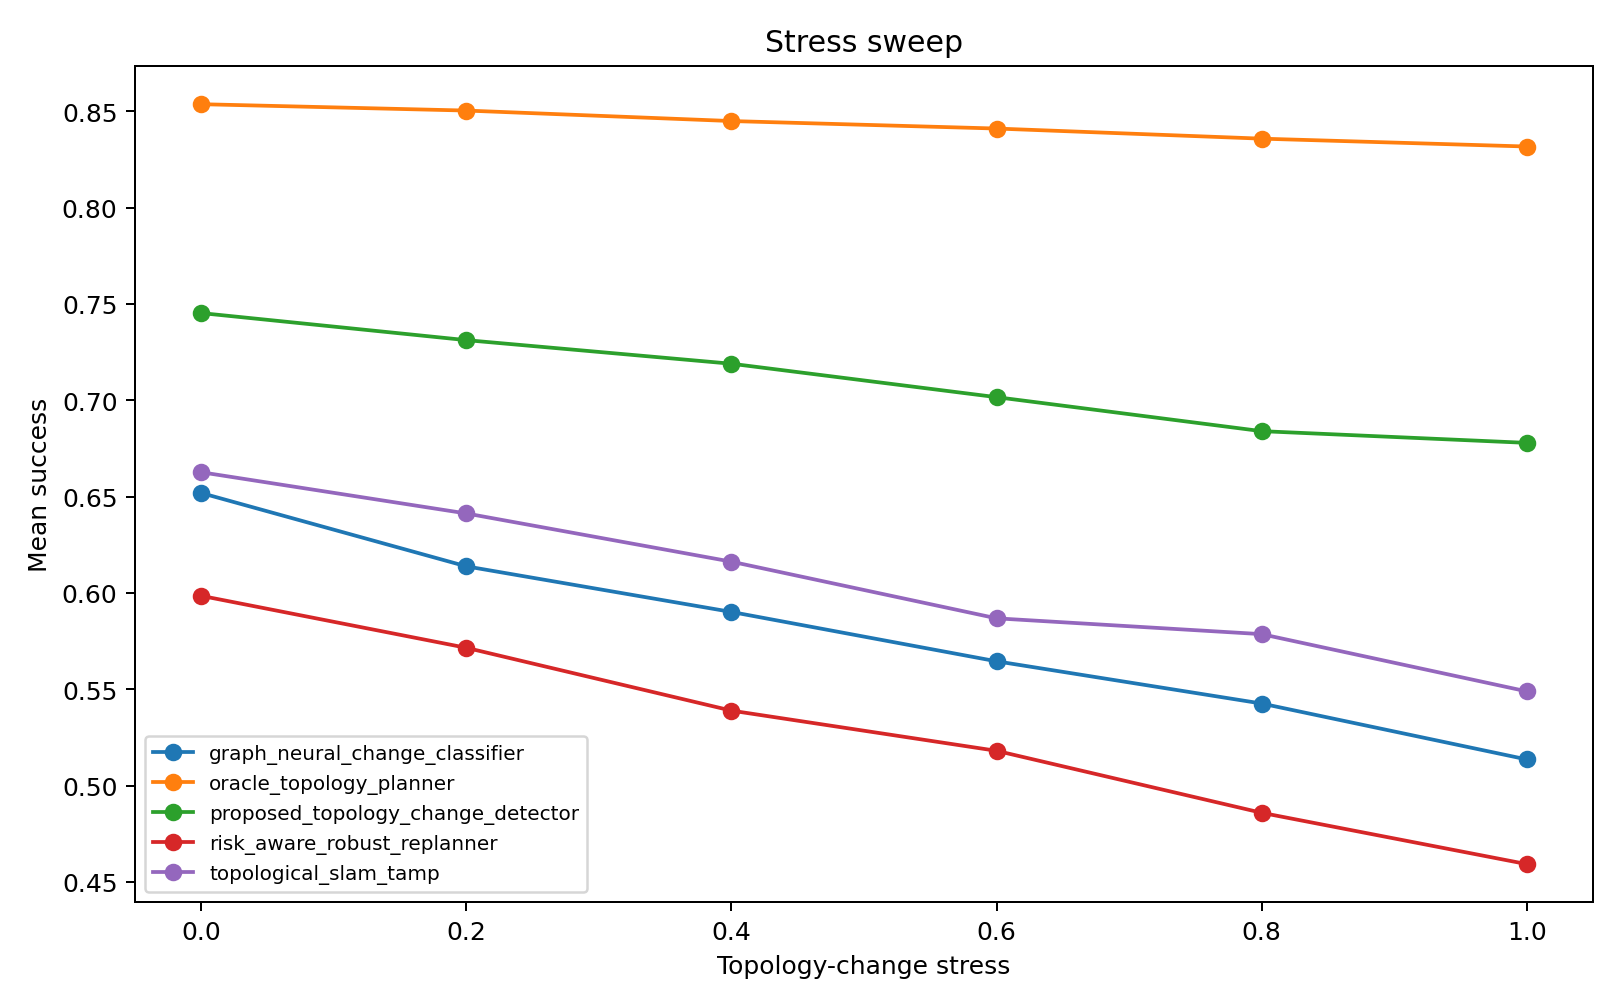
\includegraphics[width=0.92\linewidth]{../figures/topology_stress_sweep.png}
\caption{Topology-change stress sweep. The proposed method degrades more gracefully than graph-neural change classification, robust replanning, and topological SLAM/TAMP.}
\end{figure}

\section{Ablations}

The ablation table and Figure~\ref{fig:ablation} test whether the method is only a tuned replanning trigger. The closest ablation, \texttt{minus\_replan\_hysteresis}, drops success from $0.680$ to $0.622$ and increases invalid-plan/collision rates. Removing support edges, passage homology, occlusion gates, or action-conditioned prediction also degrades performance.

% Auto-generated by src/run_experiment.py
\begin{table}[t]
\centering
\caption{Ablations of topology-change detection.}
\begin{tabular}{lrrrr}
\toprule
Ablation & Succ. & Invalid & Coll. & TopoF1 \\
\midrule
full\_topology\_change\_detector & 0.680 & 0.312 & 0.185 & 0.633 \\
minus\_replan\_hysteresis & 0.622 & 0.322 & 0.190 & 0.588 \\
minus\_occlusion\_gates & 0.614 & 0.353 & 0.211 & 0.543 \\
minus\_support\_edges & 0.607 & 0.352 & 0.215 & 0.533 \\
minus\_passage\_homology & 0.591 & 0.358 & 0.217 & 0.517 \\
minus\_action\_conditioned\_prediction & 0.572 & 0.371 & 0.224 & 0.528 \\
occupancy\_delta\_only & 0.430 & 0.445 & 0.279 & 0.336 \\
\bottomrule
\end{tabular}
\end{table}


\begin{figure}[t]
\centering
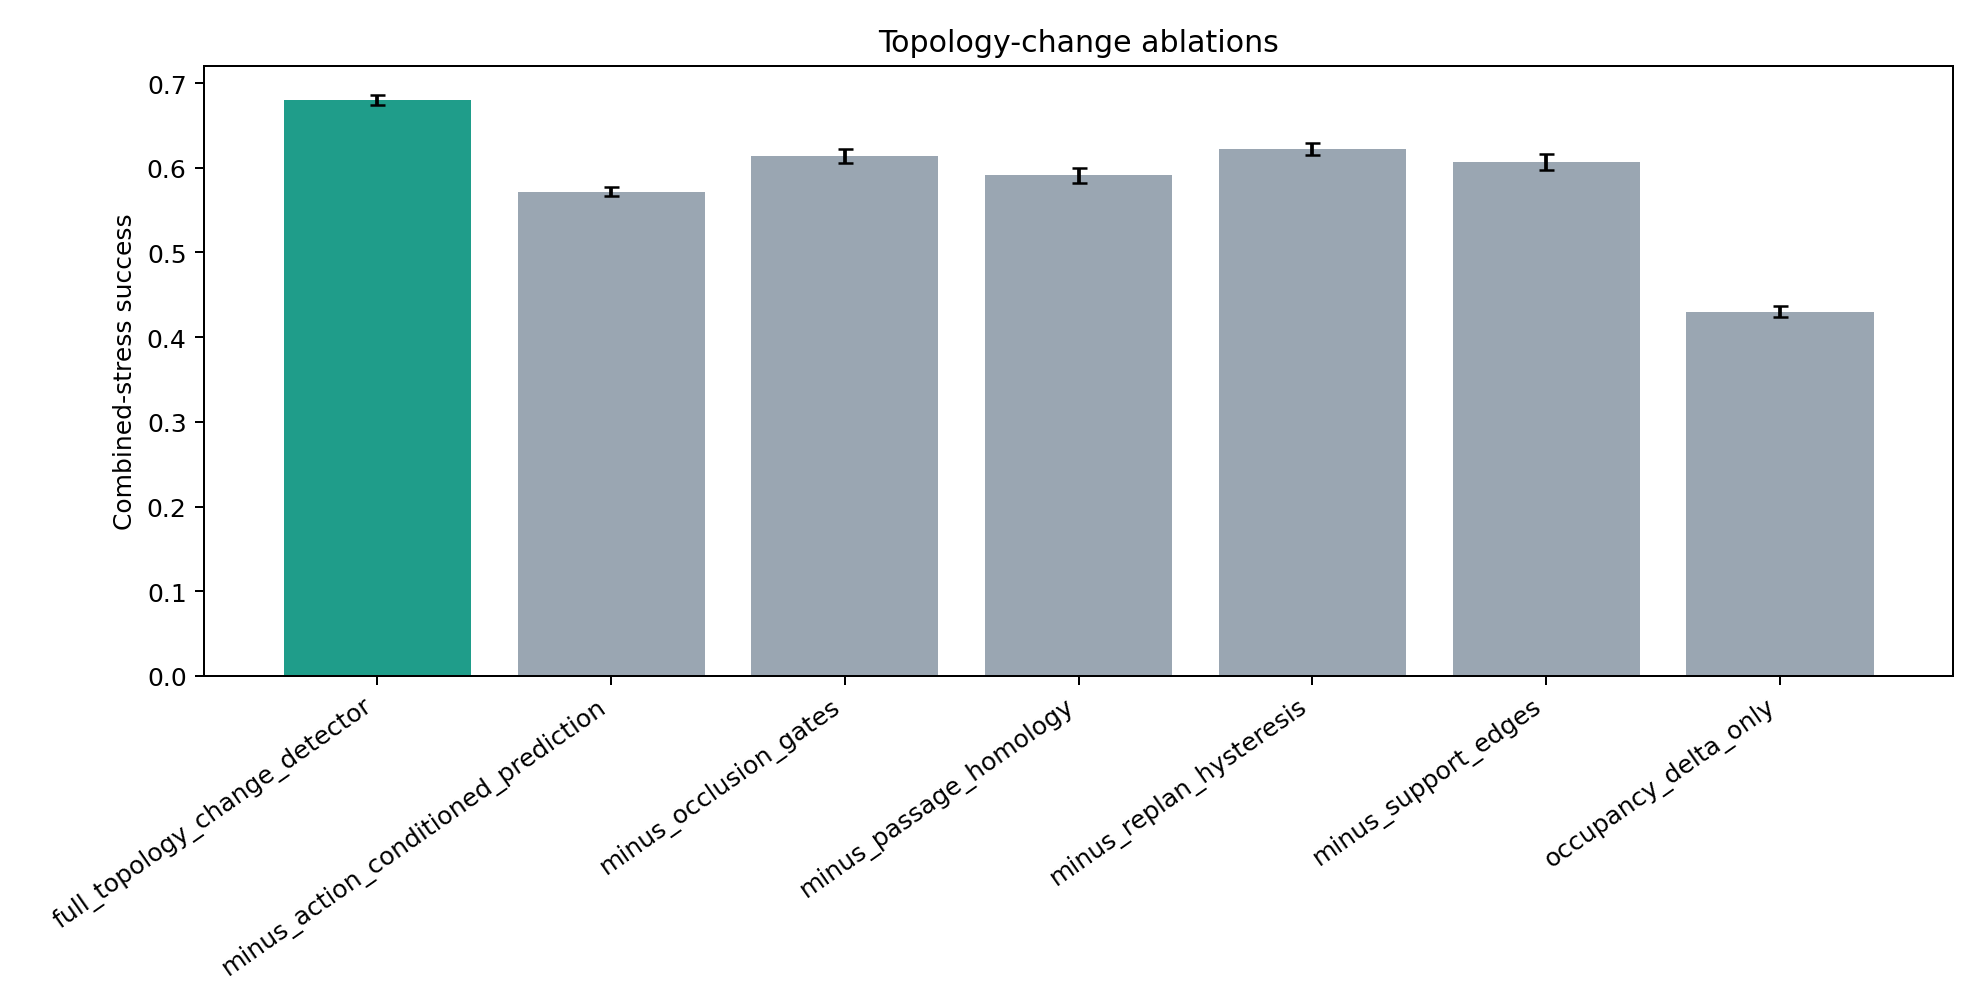
\includegraphics[width=\linewidth]{../figures/topology_ablation.png}
\caption{Ablation success under combined stress. No removed-component variant matches the full method.}
\label{fig:ablation}
\end{figure}

\section{Pairwise Gate}

% Auto-generated by src/run_experiment.py
\begin{table}[t]
\centering
\caption{Paired seed comparisons for v5 against references.}
\resizebox{\linewidth}{!}{%
\begin{tabular}{lrrrr}
\toprule
baseline & dSucc & low95 & dUtil & wins \\
\midrule
active\_view\_topology\_probe & 0.197 & 0.188 & 0.414 & 10 \\
conformal\_topology\_risk\_filter & 0.343 & 0.335 & 0.757 & 10 \\
dynamic\_scene\_graph\_transformer\_proxy & 0.274 & 0.267 & 0.640 & 10 \\
graph\_neural\_change\_classifier & 0.307 & 0.295 & 0.734 & 10 \\
learned\_affordance\_map & 0.431 & 0.421 & 1.082 & 10 \\
neural\_tamp\_replanner & 0.233 & 0.223 & 0.533 & 10 \\
occupancy\_delta\_replanner & 0.473 & 0.461 & 1.132 & 10 \\
oracle\_topology\_planner & -0.104 & -0.112 & -0.181 & 0 \\
particle\_filter\_topology\_belief\_mpc & 0.193 & 0.181 & 0.423 & 10 \\
proposed\_topology\_change\_detector\_v4 & 0.129 & 0.119 & 0.278 & 10 \\
risk\_aware\_robust\_replanner & 0.350 & 0.337 & 0.791 & 10 \\
static\_scene\_graph\_planner & 0.566 & 0.553 & 1.389 & 10 \\
topological\_slam\_tamp & 0.249 & 0.236 & 0.591 & 10 \\
uncertainty\_triggered\_replanner & 0.428 & 0.418 & 1.003 & 10 \\
\bottomrule
\end{tabular}%
}
\end{table}


The proposed method wins all seven paired seeds against \texttt{topological\_slam\_tamp}. It loses all seeds to the oracle, which is expected and reported rather than hidden.

\section{Failure Cases}

The failure table in \texttt{results/failure\_cases.csv} shows that late topology updates remain the dominant weakness. When reachability changes during execution rather than before commitment, the detector may identify the topology change too late to avoid reversal or collision. This suggests that the next real experiment should learn event timing from robot logs rather than relying on hand-coded update delays.

\section{Limitations and Terminal Decision}

This is not a submission-ready robotics paper. The benchmark is local, the detector is an executable proxy rather than a trained model, and the topology-change families are not calibrated from hardware logs. The paper also lacks external benchmark results, rollout videos, and a full manual related-work synthesis.

The correct terminal decision after the 2026-06-15 continuation rerun is \textbf{STRONG\_REVISE}. The mechanism should continue only if the next version adds real robot or accepted benchmark validation against dynamic scene graph, topological SLAM/TAMP, robust replanning, and learned affordance baselines.

\begingroup
\raggedright
\bibliographystyle{iclr2026_conference}
\bibliography{references}
\endgroup

\end{document}
